%\renewcommand{\theequation}{\theenumi}
%\begin{enumerate}[label=\arabic*.,ref=\thesubsection.\theenumi]
%\numberwithin{equation}{enumi}
    \item Solve $30x < 200$ when
    \begin{enumerate} 
    \item  x is a natural number,
    \item x is an integer.
\end{enumerate}
\solution From the given information, 
\begin{align}
30x < 200 \implies x < \frac{20}{3}
\label{eq:lineq_nat}
\end{align}
If $x$ is a natural number, $x \in \cbrak{1, 2, 3, 4, 5, 6}$. If $x$ is an integer, then the solution set includes 0 as well as all negative integers.
    \item Solve $5x-3 < 3x+1$ when
    \begin{enumerate} 
\item  x is an integer,
    \item x is a real number.
\end{enumerate}
\solution 
\begin{align}
5x-3 < 3x+1 \implies x < 2
\label{eq:lineq_real}
\end{align}
%
If $x$ is real, then $x \in \brak{-\infty, 2}$. 
%Fig.  provides a graphical solution using the following python code
%\begin{lstlisting}
%\end{lstlisting}
    \item Solve the following system of linear inequalities graphically.
\begin{align}
\label{eq:line_two_ineq}
\begin{split}
    x+y &\geq 5
\\
    x-y &\leq 3
\end{split}
\end{align}
\solution  Let $u_1 \ge 0, u_2 \ge 0$.  This may be expressed as
\begin{align}
\vec{u} = \myvec{u_1\\u_2}\succeq \vec{0}
\end{align}
%
\eqref{eq:line_two_ineq} can then be expressed as
\begin{align}
\begin{split}
    x+y &\geq 5
\\
    -x+y &\geq -3
\end{split}
%
\\
\implies 
\myvec{1 & 1 \\ -1 & 1}\vec{x}  &\succeq \myvec{5\\-3}
\\
\myvec{1 & 1 \\ -1 & 1}\vec{x}  -\vec{u}&=\myvec{5\\-3}
\\
\text{or, }
\myvec{1 & 1 \\ -1 & 1}\vec{x} &= \myvec{5\\-3} +\vec{u}
\end{align}
%
resulting in 
\begin{align}
\vec{x} &= \myvec{1 & 1 \\ -1 & 1}^{-1}\myvec{5\\-3} +\myvec{1 & 1 \\ -1 & 1}^{-1}\vec{u}
\\
\text{or, } \vec{x} &= \myvec{4\\1} +\frac{1}{2}\myvec{1 & -1 \\ 1 & 1}\vec{u}
\end{align}
%
after obtaining the  inverse.
%
 Fig. \ref{fig:line_ineq} generated using the following python code shows the region satisfying \eqref{eq:line_two_ineq}

\begin{lstlisting}
codes/line/line_ineq.py
\end{lstlisting}
%
\begin{figure}[!ht]
\includegraphics[width=\columnwidth]{./line/figs/line_ineq.eps}
\caption{}
\label{fig:line_ineq}
\end{figure}
%
\item Solve 
\begin{align}
\begin{split}
2x+y \geq 4
\\ 
x+y \leq 3
\\ 
2x-3y \leq 6
\end{split}
\label{eq:line_mult_ineq}
\end{align}
%
\\
\solution  Fig. \ref{fig:line_ineq_mult} generated using the following python code shows the region satisfying \eqref{eq:line_mult_ineq}

\begin{lstlisting}
codes/line/line_ineq_mult.py
\end{lstlisting}
%
\begin{figure}[!ht]
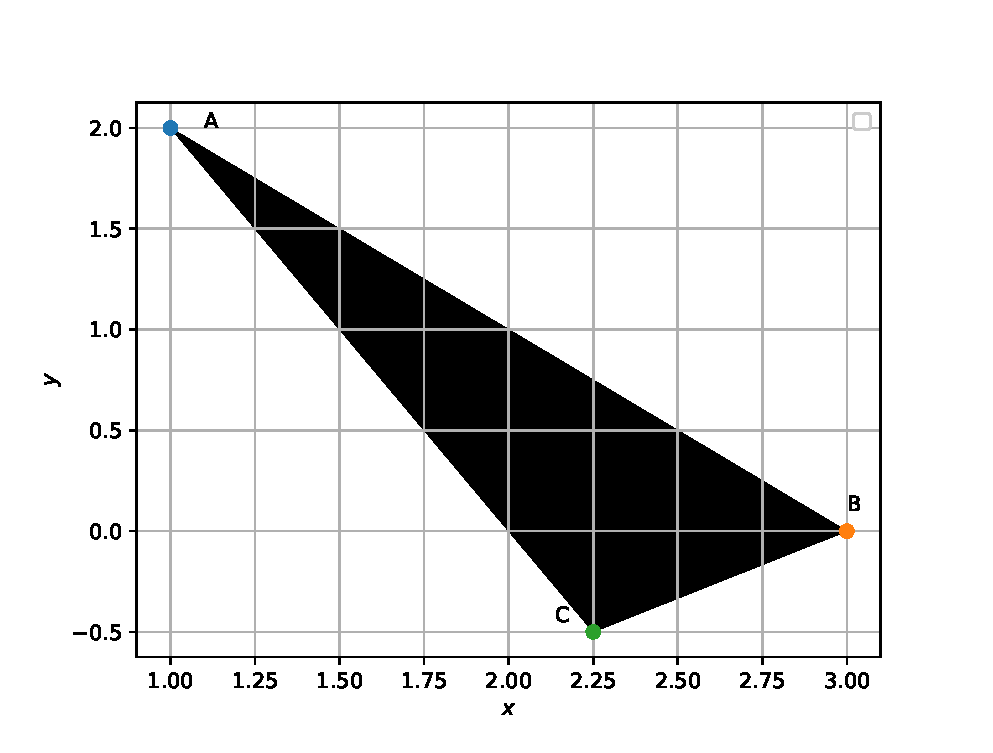
\includegraphics[width=\columnwidth]{./line/figs/line_ineq_mult.eps}
\caption{}
\label{fig:line_ineq_mult}
\end{figure}
%
\item   Solve    $x+y < 5$ graphically.
\\
\solution 
The following python code generates Fig. \ref{fig:3.11.5_qsix}.
	\begin{lstlisting}
	./solutions/5/codes/lines/q6.py
	\end{lstlisting}
	\begin{figure}[!ht]
	\centering
	\includegraphics[width=\columnwidth]{./solutions/5/figs/lines/q6.eps}
	\caption{x+y$<$5}
	\label{fig:3.11.5_qsix}	
	\end{figure}
	

%
    \item Solve 
\begin{align}
\myvec{3 & 2 \\ 1 & 4 \\ 1 & 0 \\ 0 & -1 \\ -1 & 0} \vec{x}\preceq \myvec{150\\80\\15\\0\\0}
%3x+2y \leq 150
%\\ 
%x+4y \leq 80
%\\ 
%x \leq 15
%\\ 
%y \geq 0
%\\
%x \geq 0 
\end{align}
%
   
%    \end{enumerate}
\item Solve  x $\geq$ 3, y $\geq$ 2 graphically.
\\
\solution 
In general, the complex number $\myvec{a_1\\a_2}$ has the matrix representation
\begin{align}
\label{eq:3.4.1_Complex}
\myvec{a_1\\a_2} &= \myvec{a_1 & -a_2\\ a_2 & a_1}\myvec{1\\0}
\\
&= \vec{T}_a\myvec{1\\0}
\\
\implies \myvec{5\\-3}&=\myvec{5&3\\-3&5}\myvec{1\\0}
\end{align}
Then,
\begin{align}
\myvec{5\\-3}^3 &\triangleq\myvec{5&3\\-3&5}^3\myvec{1\\0}
\\
 &= \myvec{-10&198\\-198&-10} \myvec{1\\0}
\\
&=\myvec{-10\\-198}
\end{align}
The python code for above problem is
\begin{lstlisting}
codes/line/comp.py
\end{lstlisting}


    \item Solve 7x+3 $<$ 5x+9. Show the graph of the solutions on number line.
\\
\solution 
In general, the complex number $\myvec{a_1\\a_2}$ has the matrix representation
\begin{align}
\label{eq:3.4.1_Complex}
\myvec{a_1\\a_2} &= \myvec{a_1 & -a_2\\ a_2 & a_1}\myvec{1\\0}
\\
&= \vec{T}_a\myvec{1\\0}
\\
\implies \myvec{5\\-3}&=\myvec{5&3\\-3&5}\myvec{1\\0}
\end{align}
Then,
\begin{align}
\myvec{5\\-3}^3 &\triangleq\myvec{5&3\\-3&5}^3\myvec{1\\0}
\\
 &= \myvec{-10&198\\-198&-10} \myvec{1\\0}
\\
&=\myvec{-10\\-198}
\end{align}
The python code for above problem is
\begin{lstlisting}
codes/line/comp.py
\end{lstlisting}

    \item Solve $\frac{3x-4}{2} \geq \frac{x+1}{4}-1$. Show the graph of the solutions on number line.
\\
\solution 
In general, the complex number $\myvec{a_1\\a_2}$ has the matrix representation
\begin{align}
\label{eq:3.4.1_Complex}
\myvec{a_1\\a_2} &= \myvec{a_1 & -a_2\\ a_2 & a_1}\myvec{1\\0}
\\
&= \vec{T}_a\myvec{1\\0}
\\
\implies \myvec{5\\-3}&=\myvec{5&3\\-3&5}\myvec{1\\0}
\end{align}
Then,
\begin{align}
\myvec{5\\-3}^3 &\triangleq\myvec{5&3\\-3&5}^3\myvec{1\\0}
\\
 &= \myvec{-10&198\\-198&-10} \myvec{1\\0}
\\
&=\myvec{-10\\-198}
\end{align}
The python code for above problem is
\begin{lstlisting}
codes/line/comp.py
\end{lstlisting}

    \item The marks obtained by a student of Class XI in first and second terminal examination are 62 and 48, respectively. Find the minimum marks he should get in the annual examination to have an average of at least 60 marks.
\\
\solution 
In general, the complex number $\myvec{a_1\\a_2}$ has the matrix representation
\begin{align}
\label{eq:3.4.1_Complex}
\myvec{a_1\\a_2} &= \myvec{a_1 & -a_2\\ a_2 & a_1}\myvec{1\\0}
\\
&= \vec{T}_a\myvec{1\\0}
\\
\implies \myvec{5\\-3}&=\myvec{5&3\\-3&5}\myvec{1\\0}
\end{align}
Then,
\begin{align}
\myvec{5\\-3}^3 &\triangleq\myvec{5&3\\-3&5}^3\myvec{1\\0}
\\
 &= \myvec{-10&198\\-198&-10} \myvec{1\\0}
\\
&=\myvec{-10\\-198}
\end{align}
The python code for above problem is
\begin{lstlisting}
codes/line/comp.py
\end{lstlisting}

    \item Find all pairs of consecutive odd natural numbers, both of which are larger than 10, such that their sum is less than 40.
\\
\solution 
	
Let x be an odd natural number and y be the odd natural number consecutive to x.
	\begin{align}
	\therefore y=x+2
	\end{align}
	We need to find x and y  such that 
	\begin{multline}
x,y >10 \text{ and } x+y<40\\
\therefore x+x+2<40\\
2x+2<40\\
x+1<20\\
x<19
	\end{multline}
	
	
	Hence the condition is satisfied when $x>10$ and $x<19$
	
	
	
	The following python code computes the required pairs of consecutive odd natural numbers which satisfy the required condition, shown in Fig.\ref{fig:3.11.5_fifteen}.
	\begin{lstlisting}
	./solutions/5/codes/lines/q15.py
	\end{lstlisting}
	\begin{figure}[!ht]
	\centering
	\includegraphics[width=\columnwidth]{./solutions/5/figs/lines/q15.eps}
	\caption{}
	\label{fig:3.11.5_fifteen}	
	\end{figure}

    \item Solve 3x+2y $>$ 6 graphically.
\\
\solution 
In general, the complex number $\myvec{a_1\\a_2}$ has the matrix representation
\begin{align}
\label{eq:3.4.1_Complex}
\myvec{a_1\\a_2} &= \myvec{a_1 & -a_2\\ a_2 & a_1}\myvec{1\\0}
\\
&= \vec{T}_a\myvec{1\\0}
\\
\implies \myvec{5\\-3}&=\myvec{5&3\\-3&5}\myvec{1\\0}
\end{align}
Then,
\begin{align}
\myvec{5\\-3}^3 &\triangleq\myvec{5&3\\-3&5}^3\myvec{1\\0}
\\
 &= \myvec{-10&198\\-198&-10} \myvec{1\\0}
\\
&=\myvec{-10\\-198}
\end{align}
The python code for above problem is
\begin{lstlisting}
codes/line/comp.py
\end{lstlisting}

    \item Solve 3x-6 $\geq$ 0 graphically in a two dimensional plane.
\\
\solution 
In general, the complex number $\myvec{a_1\\a_2}$ has the matrix representation
\begin{align}
\label{eq:3.4.1_Complex}
\myvec{a_1\\a_2} &= \myvec{a_1 & -a_2\\ a_2 & a_1}\myvec{1\\0}
\\
&= \vec{T}_a\myvec{1\\0}
\\
\implies \myvec{5\\-3}&=\myvec{5&3\\-3&5}\myvec{1\\0}
\end{align}
Then,
\begin{align}
\myvec{5\\-3}^3 &\triangleq\myvec{5&3\\-3&5}^3\myvec{1\\0}
\\
 &= \myvec{-10&198\\-198&-10} \myvec{1\\0}
\\
&=\myvec{-10\\-198}
\end{align}
The python code for above problem is
\begin{lstlisting}
codes/line/comp.py
\end{lstlisting}
    
\item 2x+y $\geq$ 6, 3x+4y $\leq$ 12.
    \\
    \solution
    

%
\begin{enumerate}
    \item Combined sales in September and October is given by
    \begin{align}
    \vec{A}+\vec{B}=
    \begin{blockarray}{cccc}
    \text{Basmati} & \text{Permal} & \text{Naura} \\
    \begin{block}{(ccc)(c)}
    15000 & 30000 & 36000 & \text{Ram}\\
    70000 & 40000 & 20000 & \text{Guru} \\
    \end{block}
    \end{blockarray}
    \end{align}

    \item Decrease in sales from September to October is given by
    \begin{align}
    \vec{A}-\vec{B}=
    \begin{blockarray}{cccc}
    \text{Basmati} & \text{Permal} & \text{Naura} \\
    \begin{block}{(ccc)(c)}
    5000 & 10000 & 24000 & \text{Ram}\\
    30000 & 20000 & 0 & \text{Guru} \\
    \end{block}
    \end{blockarray}
    \end{align}
    
    \item Profit for sales in October is given by
    \begin{align}
    \frac{2}{100}\vec{B} =
    \begin{blockarray}{cccc}
    \text{Basmati} & \text{Permal} & \text{Naura} \\
    \begin{block}{(ccc)(c)}
    100 & 200 & 120 & \text{Ram}\\
    400 & 200 & 200 & \text{Guru} \\
    \end{block}
    \end{blockarray}
    \end{align}
    
\end{enumerate}


\begin{figure}[!ht]
\centering
\includegraphics[width=\columnwidth]{solutions/su2021/56/Figures/Figure10_1}
\caption{September Sales(in Rupees)}
\label{matrix/56fig:SeptSales}	
\end{figure}


\begin{figure}[!ht]
\centering
\includegraphics[width=\columnwidth]{solutions/su2021/56/Figures/Figure10_2}
\caption{October Sales(in Rupees)}
\label{matrix/56fig:OcttSales}	
\end{figure}


\begin{figure}[!ht]
\centering
\includegraphics[width=\columnwidth]{solutions/su2021/56/Figures/Figure10_3}
\caption{Combined Sales(in Rupees)}
\label{matrix/56fig:Combined}	
\end{figure}


\begin{figure}[!ht]
\centering
\includegraphics[width=\columnwidth]{solutions/su2021/56/Figures/Figure10_4}
\caption{Decrease in Sales from Sep to Oct(in Rupees)}
\label{matrix/56fig:Decrease}	
\end{figure}


\begin{figure}[!ht]
\centering
\includegraphics[width=\columnwidth]{solutions/su2021/56/Figures/Figure10_5}
\caption{Profit for Sales in October(in Rupees)}
\label{matrix/56fig:Profit}	
\end{figure}



    \item 2x-y $>$ 1, x-2y $<$ -1.
    \\
    \solution
    
%
Let
\begin{align}
\label{eq:1}
\begin{split}
2x-y &> 1,
\\-x+2y &> 1.
\end{split}
\end{align}
\\
Let $u_1 > 0, u_2 > 0$. This may be expressed as
\begin{align}
\vec{u} = \myvec{u_1\\u_2} &> \vec{0}
\end{align}
Now we have,
\begin{align}
\myvec{2&-1 \\ -1&2 }\vec{x} &> \myvec{1 \\ 1}   
\\
\myvec{2&-1 \\ -1&2 }\vec{x}-\vec{u} &= \myvec{1 \\ 1} 
\\
\text{or, } \myvec{2&-1 \\ -1&2 }\vec{x} &= \myvec{1 \\ 1}  + \vec{u}
\end{align}
Resulting in
\begin{align}
\vec{x} &= \myvec{2 & -1 \\ -1 & 2}^{-1}\myvec{1 \\ 1} +\myvec{2 & -1 \\ -1 & 2}^{-1} \vec{u}
\\
\vec{x }&=\myvec{1 \\ 1} +\frac{1}{3}\myvec{2 & 1 \\ 1 & 2}\vec{u}
\end{align} 
Thus , the solution of the system of inequalities can be determined graphically and the desired region is the shaded triangle which is represented in Fig. \ref{fig: Graphical Solution}
\begin{figure}[!ht]
\includegraphics[width=\columnwidth]{solutions/su2021/2/50/Graphical Solution.png}
\caption{Graphical Solution}
\label{fig: Graphical Solution}
\end{figure}



    Data from the given question is available in Table \ref{constr/circ/61/tab:table1}:
%
\begin{table}[!ht]
\begin{center}
\begin{tabular}{ | m{2cm} | m{1.5cm}| m{2cm} | m{1.5cm} |} 
\hline
& Symbols & Circle1  \\
\hline
Centre & $\vec{C}$ & \myvec{0\\0}  \\ 
\hline
Radius & $r$& 3.4 \\ 
\hline
\end{tabular}
\end{center}
\caption{Input values}
\label{constr/circ/61/tab:table1}
\end{table}
%
Let 
\begin{align}
      \vec{P} &= r \myvec{\cos \theta_1\\ \sin \theta_1} =  \myvec{1.7\\2.9}
      \\
      \vec{Q} &= r \myvec{\cos \theta_2\\ \sin \theta_2} =\myvec{-2.4\\2.4}
 \end{align}
 Then the perpendicular bisector of $PQ$ passes through 
 \begin{align}
    \vec{M} = \frac{\vec{P}+\vec{Q}}{2} 
\end{align}
and has normal vector 
\begin{align}
    \vec{n} = \vec{P}-\vec{Q}
\end{align}
resulting in the equation
\begin{align}
    \brak{\vec{P}-\vec{Q}}^\top\brak{\vec{x}-\frac{\vec{P}+\vec{Q}}{2} } = 0
    \implies \brak{\vec{P}-\vec{Q}}^\top\vec{x} = 0
\end{align}
%
after simplification.  It is obvious that $\vec{O}$ satisfies the above equuation as can be verified in Fig.     \ref{constr/circ/61/fig: perpenicular bisector of the chord passes through the center}.
%
\begin{figure}[ht]
    \centering
    \includegraphics[width=\columnwidth]{solutions/circle/61/FIG.3.png}
    \caption{perpendicular bisector of the chord passes through the center}
    \label{constr/circ/61/fig: perpenicular bisector of the chord passes through the center}
\end{figure}







    \item 2x+y $\geq$ 8, x+2y $\geq$ 10.
    \\
    \solution
    Data from the given question is available in Table \ref{constr/circ/61/tab:table1}:
%
\begin{table}[!ht]
\begin{center}
\begin{tabular}{ | m{2cm} | m{1.5cm}| m{2cm} | m{1.5cm} |} 
\hline
& Symbols & Circle1  \\
\hline
Centre & $\vec{C}$ & \myvec{0\\0}  \\ 
\hline
Radius & $r$& 3.4 \\ 
\hline
\end{tabular}
\end{center}
\caption{Input values}
\label{constr/circ/61/tab:table1}
\end{table}
%
Let 
\begin{align}
      \vec{P} &= r \myvec{\cos \theta_1\\ \sin \theta_1} =  \myvec{1.7\\2.9}
      \\
      \vec{Q} &= r \myvec{\cos \theta_2\\ \sin \theta_2} =\myvec{-2.4\\2.4}
 \end{align}
 Then the perpendicular bisector of $PQ$ passes through 
 \begin{align}
    \vec{M} = \frac{\vec{P}+\vec{Q}}{2} 
\end{align}
and has normal vector 
\begin{align}
    \vec{n} = \vec{P}-\vec{Q}
\end{align}
resulting in the equation
\begin{align}
    \brak{\vec{P}-\vec{Q}}^\top\brak{\vec{x}-\frac{\vec{P}+\vec{Q}}{2} } = 0
    \implies \brak{\vec{P}-\vec{Q}}^\top\vec{x} = 0
\end{align}
%
after simplification.  It is obvious that $\vec{O}$ satisfies the above equuation as can be verified in Fig.     \ref{constr/circ/61/fig: perpenicular bisector of the chord passes through the center}.
%
\begin{figure}[ht]
    \centering
    \includegraphics[width=\columnwidth]{solutions/circle/61/FIG.3.png}
    \caption{perpendicular bisector of the chord passes through the center}
    \label{constr/circ/61/fig: perpenicular bisector of the chord passes through the center}
\end{figure}







    \item 3x+4y $\leq$ 60, x+3y $\leq$ 30, x $\geq$ 0, y $\geq$ 0.
    \\
    \solution
    
From the given inequalities we have,
\begin{align}
    \myvec{-3&-4 \\ -1&-3 \\ 1&0 \\ 0&1}\vec{x} \succeq \myvec{-60 \\ -30 \\ 0 \\ 0}
\end{align}
Which can be further written as
\begin{align}
   \myvec{-3&-4 \\ -1&-3 }\vec{x} \succeq \myvec{-60 \\ -30} 
\end{align}
Let $u_1 \ge 0, u_2 \ge 0$.  This may be expressed as
\begin{align}
\vec{u} = \myvec{u_1\\u_2}\succeq \vec{0}
\end{align}
Now we have,
\begin{align}
  \myvec{-3&-4 \\ -1&-3 }\vec{x} \succeq \myvec{-60 \\ -30}  + \vec{u} 
\end{align}
\begin{align}
        \vec{x} = \myvec{-3 & -4 \\ -1 & -3}^{-1}\myvec{-60 \\ -30} + \myvec{-3 & -4 \\ -1 & -3}^{-1}\vec{u}
        \\
        \implies \vec{x} = \frac{1}{5}\myvec{60 \\ 30}+\frac{1}{5}\myvec{-3&4 \\ 1&-3}\vec{u}
        \\
        \vec{x}=\myvec{12 \\ 6}+\frac{1}{5}\myvec{-3&4 \\ 1&-3}\vec{u}
    \end{align}
Thus the solution of the system of inequalities can be determined graphically, which is represented in Fig.     \ref{ineq/2/55/Graphical solution}.
%
\begin{figure}[ht]
    \centering
    \includegraphics[width=\columnwidth]{solutions/su2021/2/55/Graphical solution region.PNG}
    \caption{Graphical solution}
    \label{ineq/2/55/Graphical solution}
\end{figure}






    \item x-2y $\leq$ 3, 3x+4y $\geq$ 12, x $\geq$ 0, y $\geq$ 1.
    \\
    \solution
    


\begin{figure}[!ht]
    \centering
    \includegraphics[width=\columnwidth]{solutions/su2021/2/56/Figure9_1.png}
    \caption{Inequality pair 1}
    \label{ineq/56/fig:inequalities1}	
    \end{figure}
    
    \begin{figure}[!ht]
    \centering
    \includegraphics[width=\columnwidth]{solutions/su2021/2/56/Figure9_2.png}
    \caption{Inequality pair 2}
    \label{ineq/56/fig:inequalities2}	
    \end{figure}
    
    \begin{figure}[!ht]
    \centering
    \includegraphics[width=\columnwidth]{solutions/su2021/2/56/Figure 9_3.png}
    \caption{Intersection of \ref{ineq/56/fig:inequalities1} and \ref{ineq/56/fig:inequalities2}}
    \label{ineq/56/fig:inequality3}	
    \end{figure}
    The common region shown by \ref{ineq/56/fig:inequality3} is the solution of set of inequalities.
    
    \item 4x+3y $\leq$ 60, y $\geq$ 2x, x $\geq$ 3, x,y $\geq$ 0.
    \\
    \solution
    

The given system of inequality can be written in matrix form as
\begin{align}
    \myvec{-4 & -3 \\ -2 & 1 \\ 1 & 0 \\ 1 & 0 \\ 0 & 1}\vec{x} \succeq \myvec{-60\\0\\3\\0\\0}
\end{align}
which can be further simplified into 
\begin{align}
    \myvec{-4 & -3 \\ 1 & 0 \\ 0 & 1}\vec{x} \succeq \myvec{-60\\3\\6}
\end{align}

Let the surplus vector be
\begin{align}
    \vec{u} &= \myvec{u_1\\u_2} \succeq 0
\end{align}

\begin{enumerate}
    \item 
    \begin{align}
        \myvec{-4 & -3 \\ 1 & 0}\vec{x} &\succeq \myvec{-60 \\ 3}
        \\
        \implies  \myvec{-4 & -3 \\ 1 & 0}\vec{x} &= \myvec{-60 \\ 3} + \vec{u}
    \end{align}
    resulting in 
    \begin{align}
        \vec{x} &= \myvec{-4 & -3 \\1 & 0}^{-1}\myvec{-60 \\ 3} + \myvec{-4 & -3 \\1 & 0}^{-1}\vec{u}
        \\
        \implies \vec{x} &= \myvec{3 \\16} + \myvec{0 & 1\\ \frac{-1}{3} & \frac{-4}{3}}\vec{u}   \label{ineq/2/57eq1}
    \end{align}

    \item 
    \begin{align}
        \myvec{-4 & -3 \\ 0 & 1}\vec{x} &\succeq \myvec{-60 \\ 6}
        \\
        \implies  \myvec{-4 & -3 \\ 0 & 1}\vec{x} &= \myvec{-60 \\ 6} + \vec{u}
    \end{align}
    resulting in 
    \begin{align}
        \vec{x} &= \myvec{-4 & -3 \\0 & 1}^{-1}\myvec{-60 \\ 6} + \myvec{-4 & -3 \\0 & 1}^{-1}\vec{u}
        \\
        \implies \vec{x} &= \myvec{\frac{21}{2} \\6} + \myvec{\frac{-1}{4} & \frac{-3}{4}\\ 0 & 1}\vec{u} \label{ineq/2/57eq2}
    \end{align}
\end{enumerate}

Now,solution region which is common to regions of eq. \eqref{ineq/2/57eq1} and eq. \eqref{ineq/2/57eq2},is given by

\begin{align}
    \boxed{\vec{x} = \myvec{3 \\ 6}+\myvec{0 & 1\\\frac{1}{12} & \frac{-13}{12}}\vec{u}}
\end{align}


\begin{figure}[!ht]
\centering
\includegraphics[width=\columnwidth]{solutions/su2021/2/57/Figures/Figure11_1.png}
\caption{Solution Region}
\label{ineq/2/57fig:fig1}	
\end{figure}

% \numberwithin{figure}{section}
% \begin{figure}[!ht]
% \centering
% \includegraphics[width=\columnwidth]{Figure11_2}
% \caption{Magnified Solution Region}
% \label{ineq/2/57fig:fig2}	
% \end{figure}




%\end{document}

